\section{Runtime Architecture}

\subsection{Runtime}

\begin{figure}
		\centering
		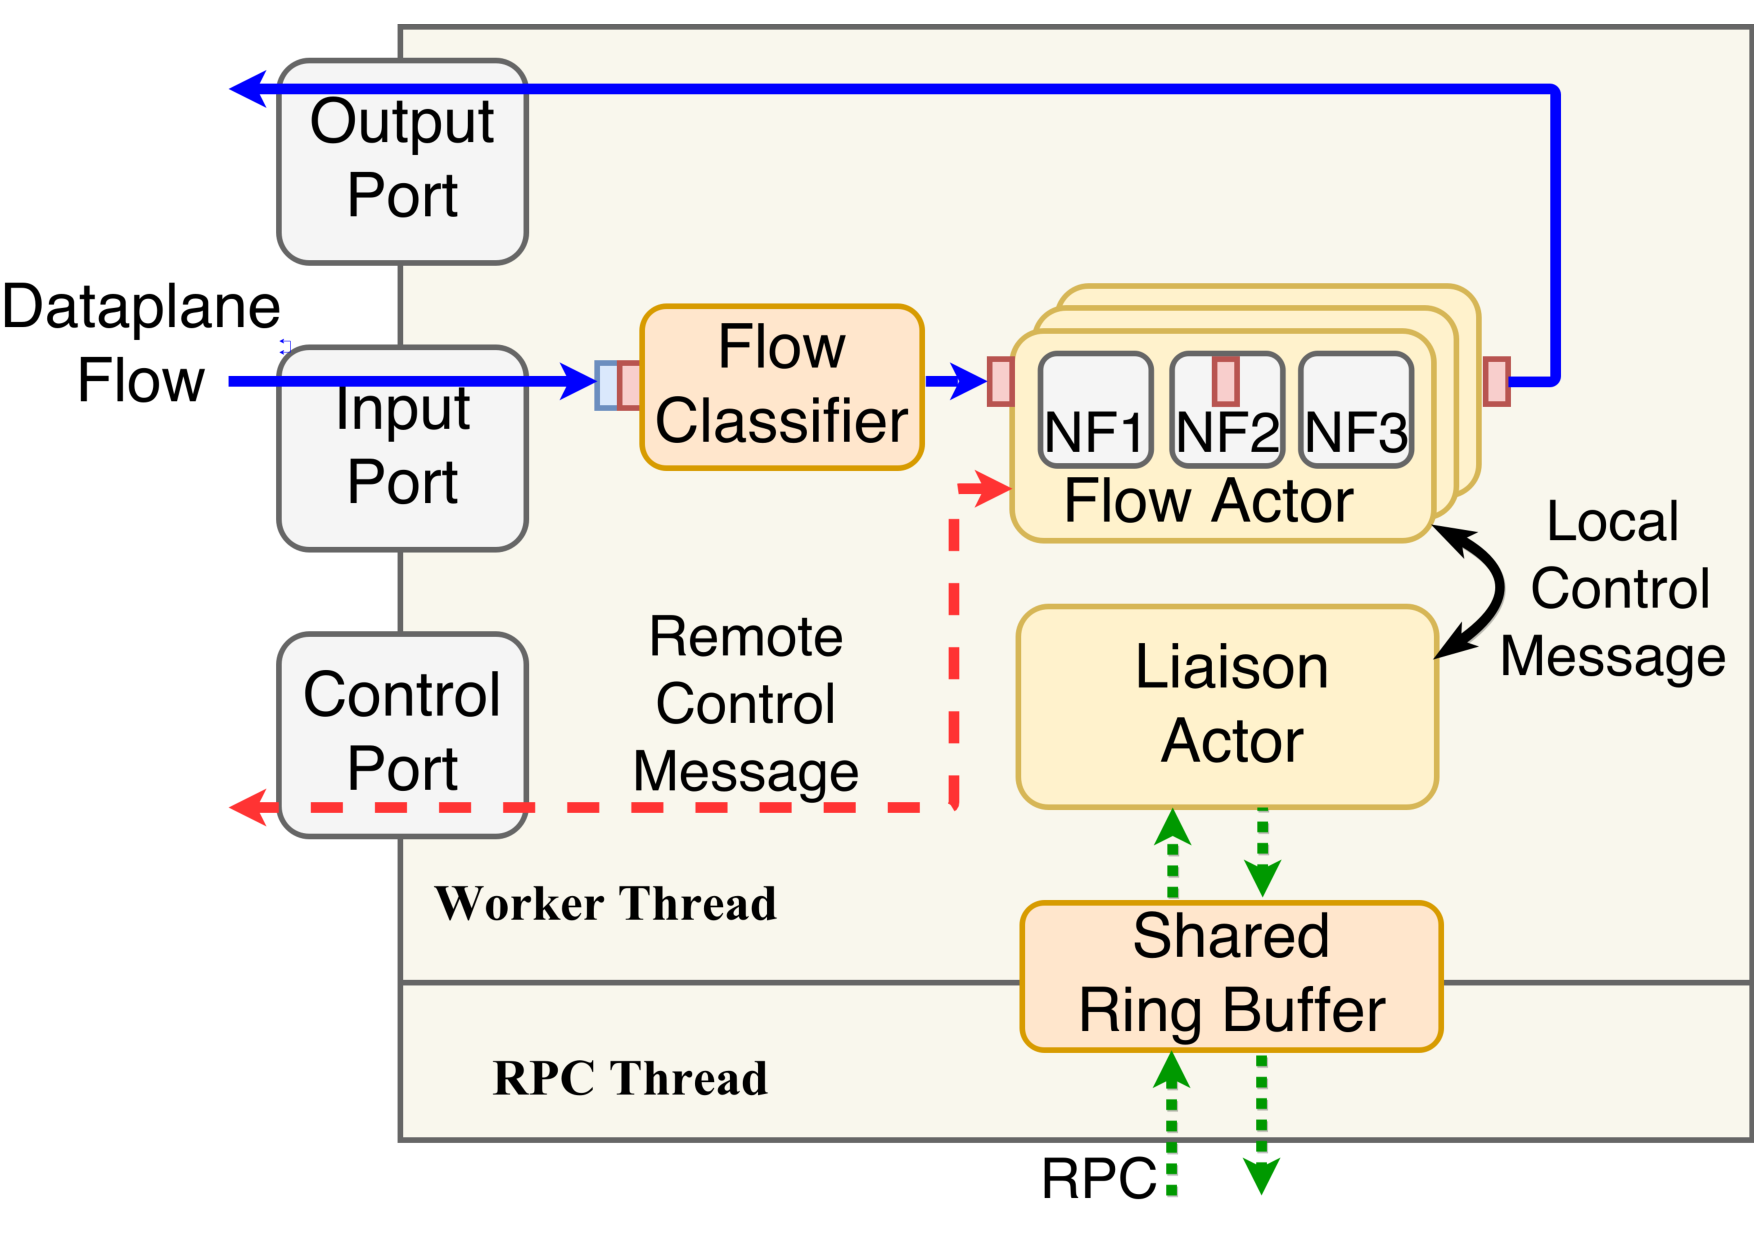
\includegraphics[width=\columnwidth]{figure/new-nfactor-runtime-arch.pdf}

		\caption{The internal architecture of a NFActor runtime system. }
\label{fig:runtime-arch}
\end{figure}

Figure \ref{fig:runtime-arch} demonstrates the internal architecture of a runtime. The runtime consists of a worker thread, which schedules actors to do service chain processing, and an RPC thread, which receives RPC requests from the controller and forwards them to the worker thread through a shared ring buffer. The runtime is configured with three ports, from which it can send and receive packets.

The worker thread polls dataplane packets from the input port and forwards the packets to a flow classifier, which uses traditional flow-5-tuple (i.e. IP destination address, IP source address, transmission layer protocol, source port and destination port) as the key to classify flows. For each new flow, the flow classifier creates an unique flow actor and forwards all the packets associated with the flow to that flow actor. The flow actor provides a micro execution context for the flow, which is configured several message handlers, including a handler for processing input packet and handlers for dealing with flow migration and replication. There is a coordinator actor who is responsible for executing the RPC requests sent from the coordinator and coordinate flow actors during flow management tasks. Flow actor and coordinator actor on the same runtime could directly pass messages with each other. Actors on different runtime use reliable message transmission module \ref{} to send remote messages over the three ports \ref{}.

The runtime is configured with a specific service chain during the boot phase and initializes all the NF modules as specified in the service chain. When a flow actor is created, it loads these modules and uses the flow state allocation method \ref{table:api} to allocates all the
To process flows across a service chain, during the initialization phase of the runtime, a service chain specifier is passed in to the runtime. The runtime then loads all the NF modules as indicated in the service chain specifier. When the flow classifier creates a new flow actor, the flow actor also loads these NF modules on the service chain and passes the input packet along the NF modules in sequence.

The reason that the runtime is designed as a single-worker-thread program is because the multi-worker-thread design may not bring significant performance gain. In our initial prototype implementation, we use LIBCAF \cite{caf} library to construct flow actors. LIBCAF library creates multiple worker threads and schedules flow actors to run on these worker threads. Because LIBCAF completely conceals the internal interfaces of the worker threads, we have to create a dedicated polling thread to poll packet from the input port. Under this design, we find that the maximum throughput of a runtime does not increase when the number of LIBCAF worker thread increases, because the polling thread has always been a bottleneck. Therefore, we abandon the multi-worker-thread design and use a single worker thread to poll packets and schedule flow actors. To our surprise, this architecture turns out to work very well because it allows us to perform aggressive optimization of actor programming model \ref{}. In the mean time, we can still maintain the scalability of the system by launching more runtimes.

\subsection{Virtual Switch}

The virtual switch is just a special runtime whose service chain is not configured during initialization time. Therefore, the flow actor created by the virtual switch does not need to do service chain processing and only performs virtual switching. Flow actors in the virtual switch are referred to as virtual switch actors throughout the rest of this paper.

When a virtual switch actor is created by the virtual switch, it selects one of the available runtimes as its destination in a round-rubin way. We use a round-rubin algorithm because the virtual switch must have good performance and round-rubin algorithm imposes the smallest overhead. Whenever the virtual switch actor receives an input packet, it replaces the destination MAC address of the input packet with the MAC address of the input port of the destination runtime, and modifies the source MAC address of the input packet into the MAC address of the output port of the virtual switch, it then sends the packet out from the output port.

The flow actor on the destination runtime could analyze the source MAC address of the packet and determine which virtual switch this packet comes from. This helps the flow actor to contact the virtual switch actor during flow migration and replication to change flow route \ref{}.

The virtual switch provides automatic load-balancing inside a NFActor cluster as shown in figure \ref{fig:runtime}, thereby improving the scalability of NFActor framework. When there is overload, the controller could launch a new runtime and the workload could be automatically balanced on that runtime. The architectural consistency of virtual switch and runtime also facilitates flow management tasks, as it enables direct communication between flow actors and virtual switch actors to dynamically change flow route \ref{} in a fully distributed fashion.

\subsection{Controller and Control RPCs}

%运行时系统暴露了一系列RPC以供controller进行调用。这些rpc可以分为以下几类:控制流管理任务的rpc仅仅

The controller in NFActor is a light-weight one. It is responsible for monitoring the workload of each runtime, executes dynamic scaling. This is similar with NFV system controllers in E2 \cite{palkar2015e2} and Stratos \cite{gember2012stratos}. The most important difference of our controller is that it only needs to participate in the initiation phase of flow migration and replication. Due to the use of actor programming model, there is no need for the controller to coordinate flow migration and replication as in OpenNF \cite{gember2015opennf} and Split/Merge \cite{rajagopalan2013split}.

The controller communicates with runtime and virtual switches using a series of control RPCs. The use of control RPCs decouples the execution of the runtime with the execution of the controller and decreases the complexity in developing the controller. The controller uses control RPCs to poll workload information and notifies virtual switches and runtimes about the configuration information of each other. The configuration information includes mac address of the input/output/control port and ID of runtime/virtual switch. Virtual switches and runtimes can use the configuration information to contact each other \ref{}.

The following three RPCs enables the controller to initiate flow management tasks. The details of these RPCs are further illustrated in \ref{}.

\begin{itemize}

\item \textbf{Migrating Flows to Migration Target Runtime.} This RPC call sets up a migration target runtime for the RPC target and indicates the number of flows to migrate. When this call finishes, the RPC target should start migrating flows to the migration target.

% 设置replication target。 为一个runtime设置replication target。replication target和当前runtime也必须处于同一个layer。当设置好replication target后,新到来的流就会被replicate到replication target上。

\item \textbf{Setting up Repliation Target Runtime.} This RPC call sets up a replication target runtime. When this call finishes, the RPC target should start replicating new flows to the replication target runtime.

% 恢复 failed runtime. 如果当前runtime 时failed runtime的replication target,那么保存在当前runtime上的flow replica就会被直接在当前runtime上恢复过来。
\item \textbf{Recovering Failed Runtime.} If the RPC target is the replication target runtime of the failed runtime, then flows replicated on the RPC target are directly recovered on the RPC target.

\end{itemize}

\subsection{Flow Management}

In NFActor, the flow management task is automatically executed by each flow actor, without the coordinator from a central controller. This feature provides good scalability when there are multiple runtimes in the cluster. Inside a NFActor cluster, each flow could do route selection by itself, therefore there is no need to rely on SDN switches and controllers. This improve the usablility and performance of NFActor framework, because SDN may not be available at all time and SDN incurs a high processing overhead when dynamically changing flow rules. Finally, the new NF modules APIs completely separate the flow state with NF processing logic. The flow actor could manipulate the flow states at any time, and the entire flow management tasks are completely transparent to the NFs. Any NF modules implemented on top of the APIs provided by NFActor could be seamlessly integrated with flow management tasks. From the perspective of NF module programmers, this feature helps them focus on the internal logic design when implementing NFs, instead of considering how to integrate their code with complicated flow management tasks. This greatly impiroves the applicability of NFActor framework. The following 2 sections give details about how flow migration and replication tasks are implemented in NFActor system.

\subsubsection{Flow Migration}

\begin{figure}[!h]
\begin{subfigure}[t]{0.33\linewidth}
   \centering
   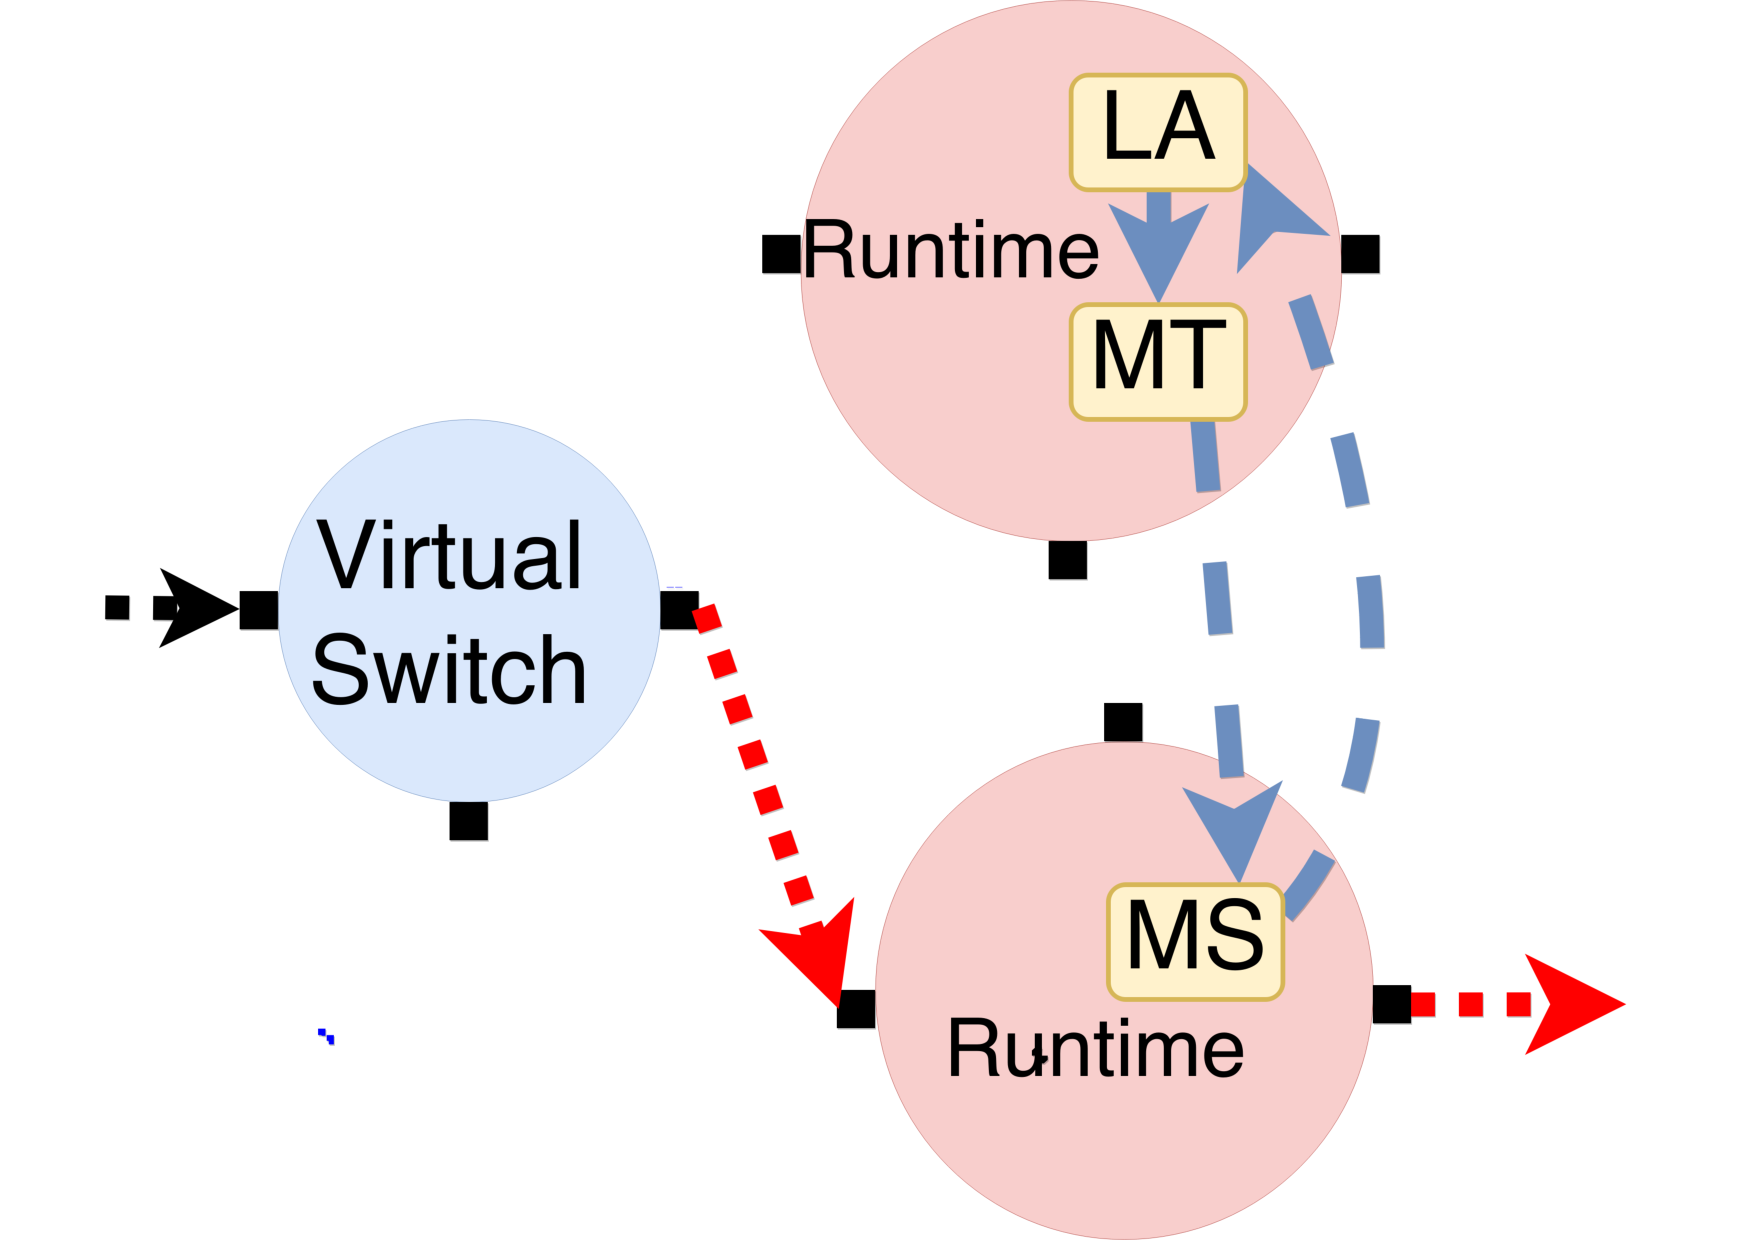
\includegraphics[width=\columnwidth]{figure/nfactor-mig1.pdf}
   \caption{1st req-rep.}\label{fig:mig1}
  \end{subfigure}\hfill
  \begin{subfigure}[t]{0.33\linewidth}
     \centering
     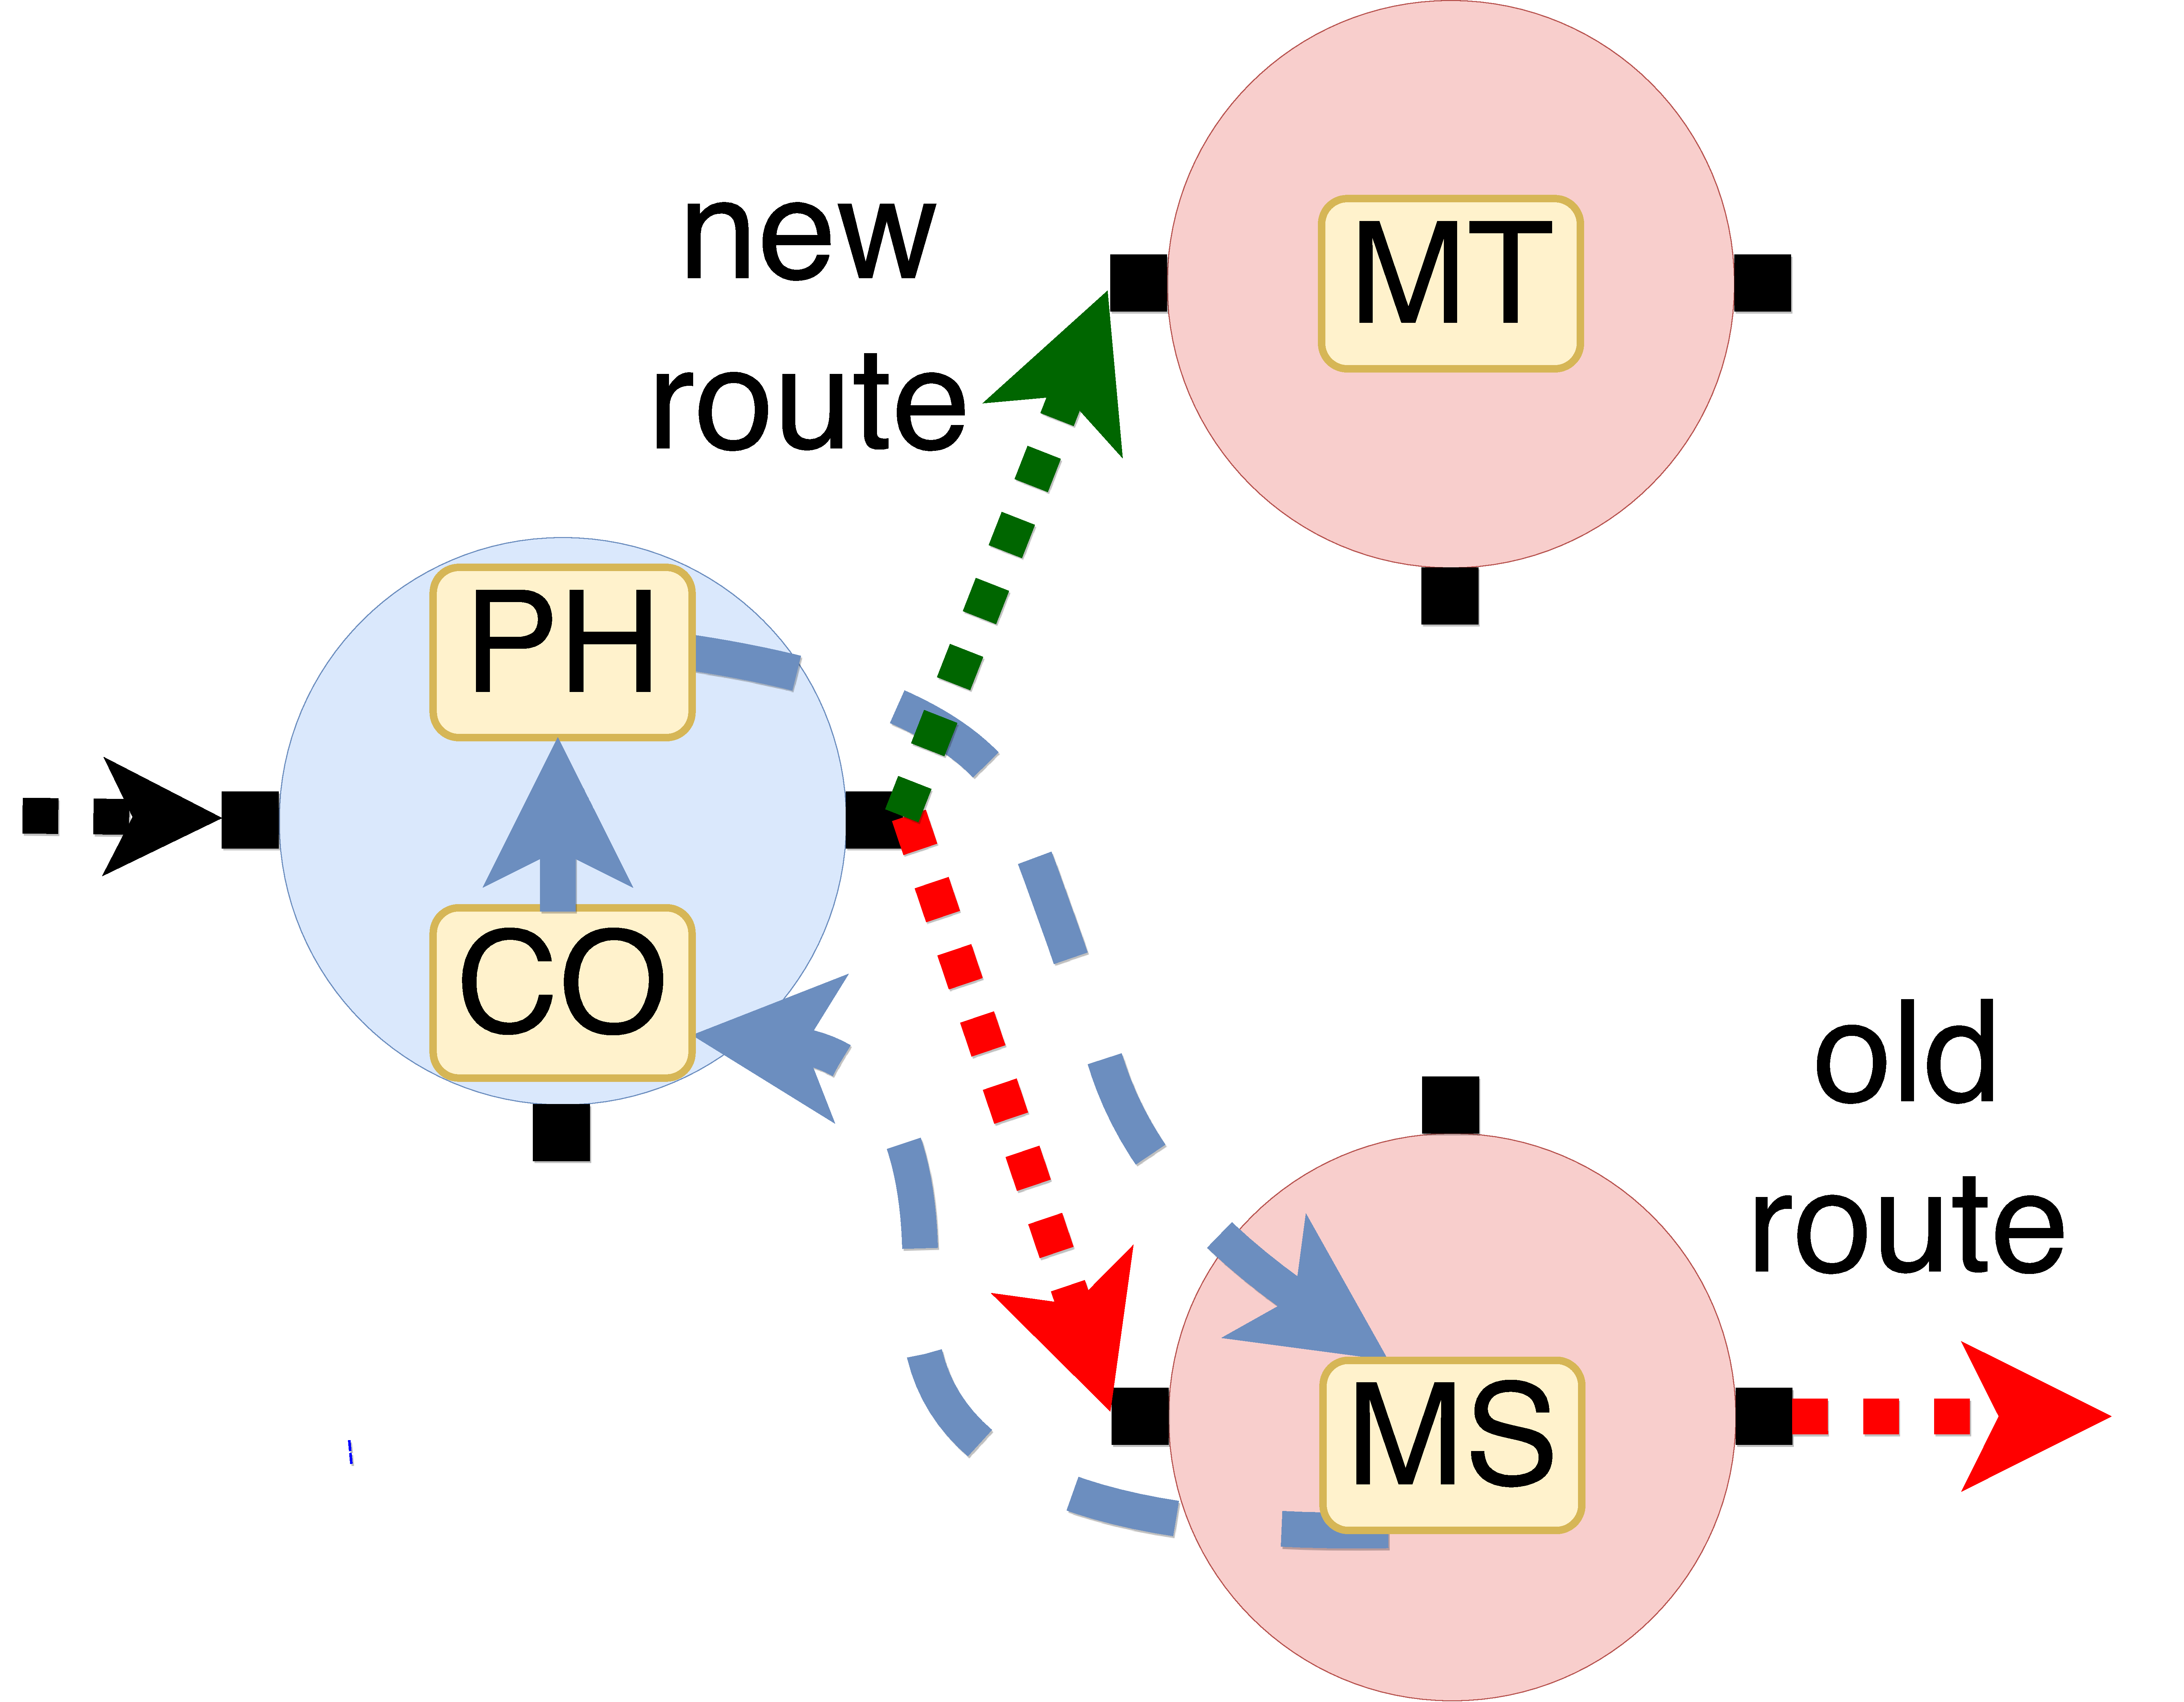
\includegraphics[width=\columnwidth]{figure/nfactor-mig2.pdf}
     \caption{2nd req-rep.}\label{fig:mig2}
    \end{subfigure}\hfill
  \begin{subfigure}[t]{0.33\linewidth}
 \centering
   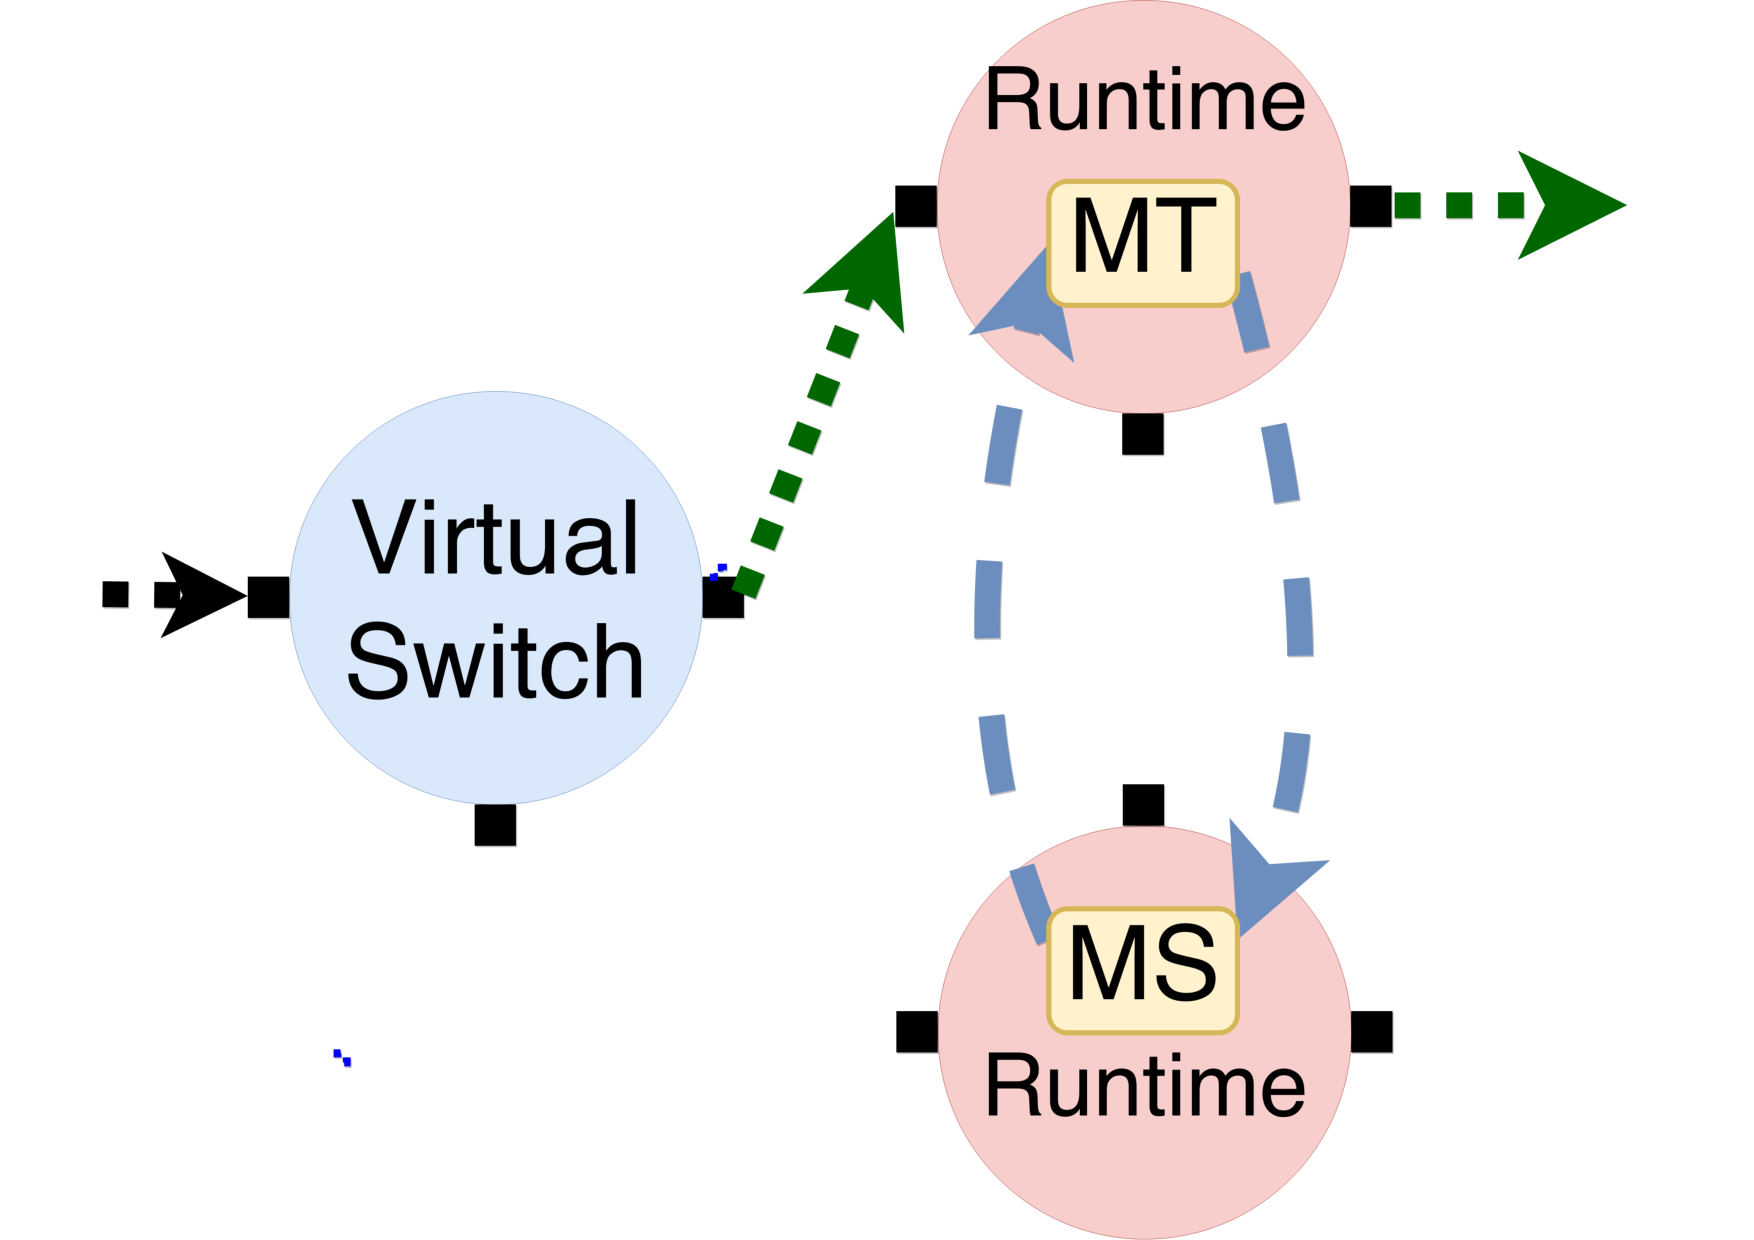
\includegraphics[width=\columnwidth]{figure/nfactor-mig3.pdf}
   \caption{3rd req-rep.}\label{fig:mig3} \end{subfigure}\hfill
 \caption{The three request-responses used during flow migration. (\textbf{MT}: Migration target actor. \textbf{MS}: Migration source actor. \textbf{CO}: Coordinator actor. \textbf{PH}: Flow actor on previous hop. \textbf{Dotted line}: Dataplane flow packets. \textbf{Dashed line}: Actor messages.)}
\label{fig:mig}
\end{figure}

As is shown in figure \ref{fig:mig}, when the current flow actor being migrated receives a migration command, it starts flow migration by executing the following three groups of request-responses.

\begin{itemize}

\item \textbf{First,} the current flow actor sends a request to the coordinator actor on the migration target runtime, containing the flow-5-tuple of the current flow actor. After receiving this request, the coordinator actor creates a migration target actor using the flow-5-tuple contained in the request. The migration taget actor then gives a response to the current flow actor.

\item \textbf{Second,} the current flow actor sends another request to the coordinator actor of its previous hop runtime, containing the flow-5-tuple and the ID of the migration target runtime. The coordinator actor uses the flow-5-tuple to find out the flow actor on the previous hop and notifies that flow actor to modify its output route to the migration target runtime. When the flow actor on previous hop finishes modifying the route, it gives a response back to the current flow actor. Also, after route modification, the migration target starts to receive data packets. The migration target actor buffers the data packets until the third group of request-response finishes.

\item \textbf{Third,} the flow actor sends its flow state to the migration target actor. After receiving the flow states, the migration target actor saves them, gives a response to the current flow actor and immediately start processing all the buffered packets. The current flow actor exits when receiving the response.

\end{itemize}

\textbf{Lossless Migration.} Even though the three request-responses are seemingly trivial, they actually achieve lossless migration as defined in OpenNF. If the three request-responses are successfully completed, the flow being migrated will not miss processing a single packet. The key reason is that when the flow actor being migrated receives the second response, it will not receive any more data plane packet sent to it anymore. This is because the second response is actually delivered by the same network path as the data plane packets. Recall that in figure \ref{fig:runtime-arch}, the remote messages could also be sent over input/output ports of a runtime. The second response is actually sent by the output port of the previous hop runtime and received by the input port of the current runtime, thereby sharing the same network path as the data plane packets. If the network does not re-order any packets (the network could indeed re-order packets, but the possibility is extremely low and there is no known method to fight agaist this kind of error) , then the current flow actor receives no more dataplane packets because the route has been changed prior to the previous hop actor sending out the second response. Therefore, no packet is missed during the migration operation.

\textbf{Error Handling.} The three request-responses may not always be successfully executed. In case of request failure, the current flow actor is responsible for restoring the modified route (if it happens) and resumes normal packet processing. The migration target actor is deleted after a timeout.

\subsubsection{Flow Replication}

\begin{figure}[!h]
\begin{subfigure}[t]{0.49\linewidth}
   \centering
   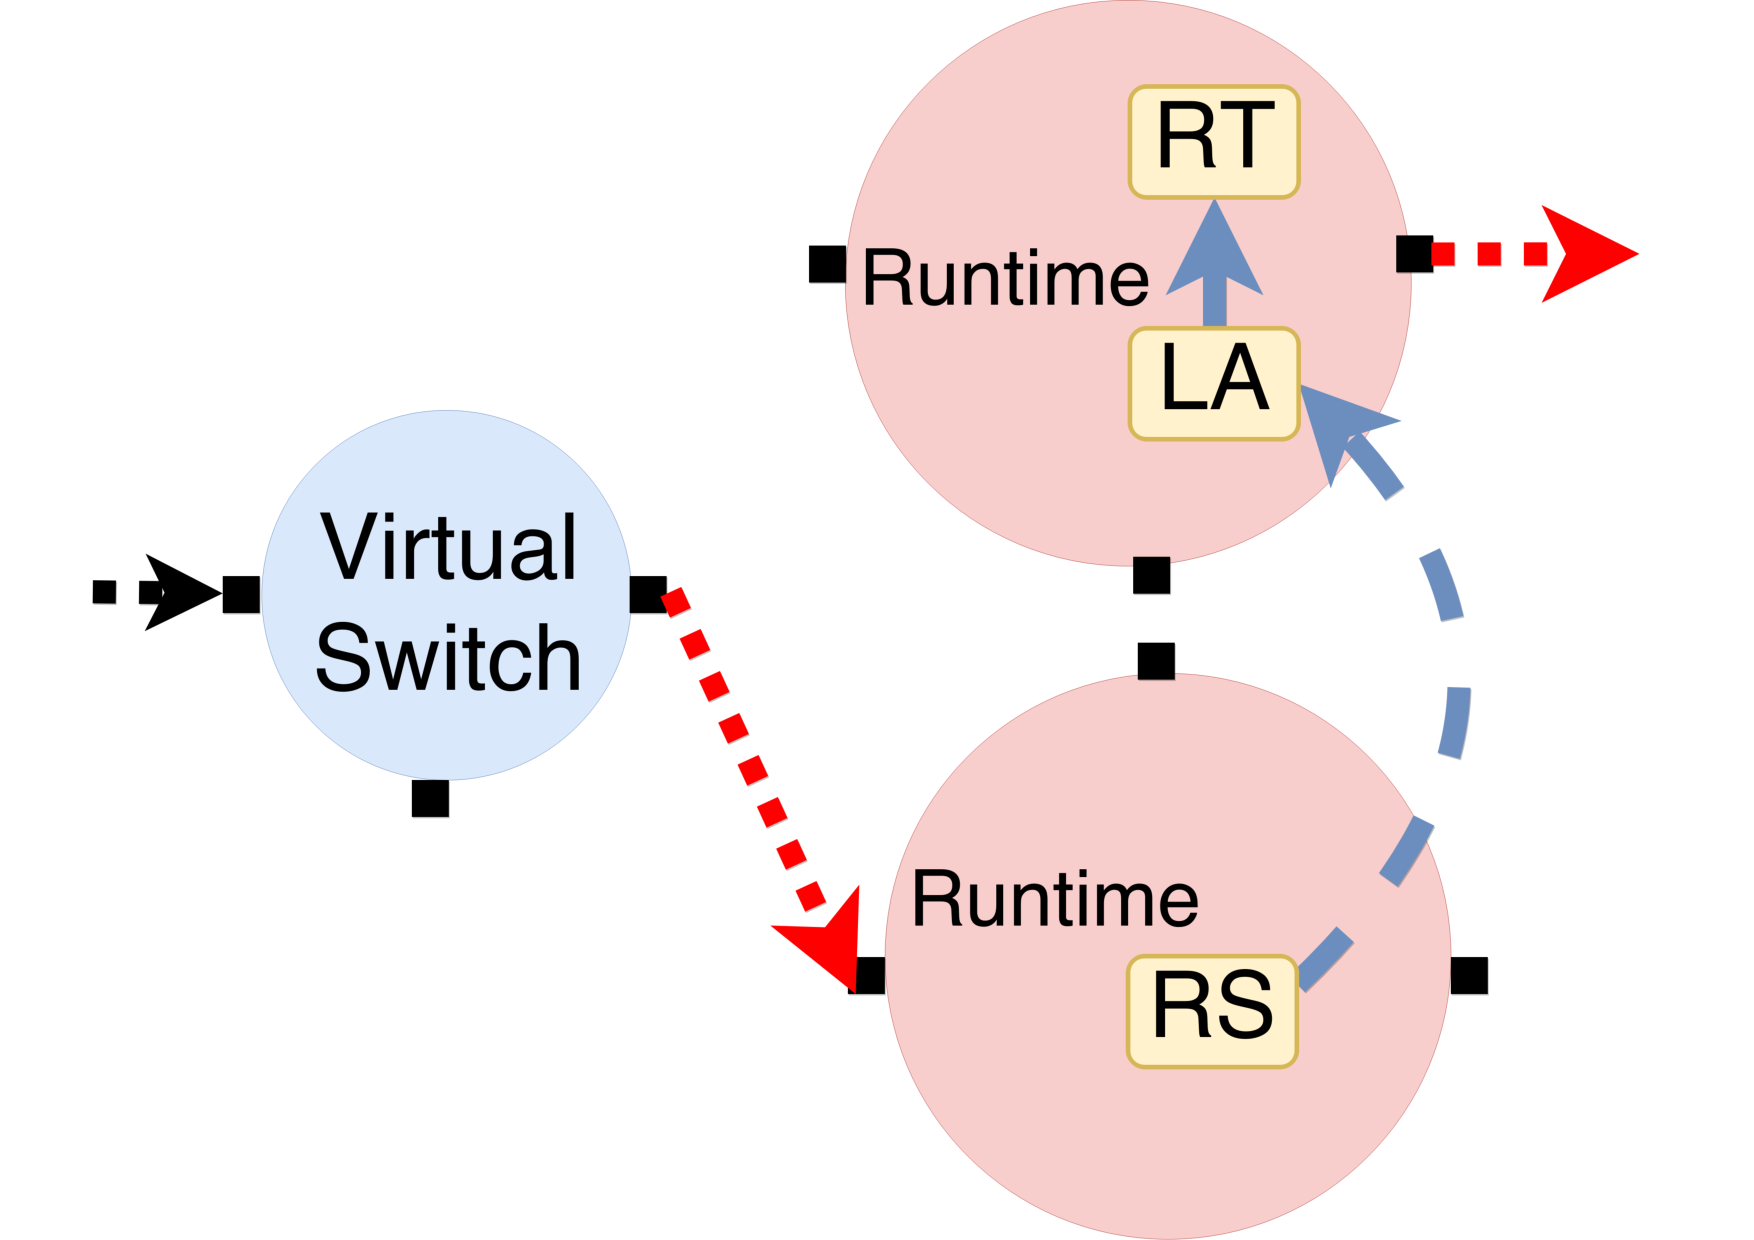
\includegraphics[width=0.66\columnwidth]{figure/nfactor-replication.pdf}
   \caption{Flow replication.}\label{fig:rep}
  \end{subfigure}
  \begin{subfigure}[t]{0.49\linewidth}
     \centering
     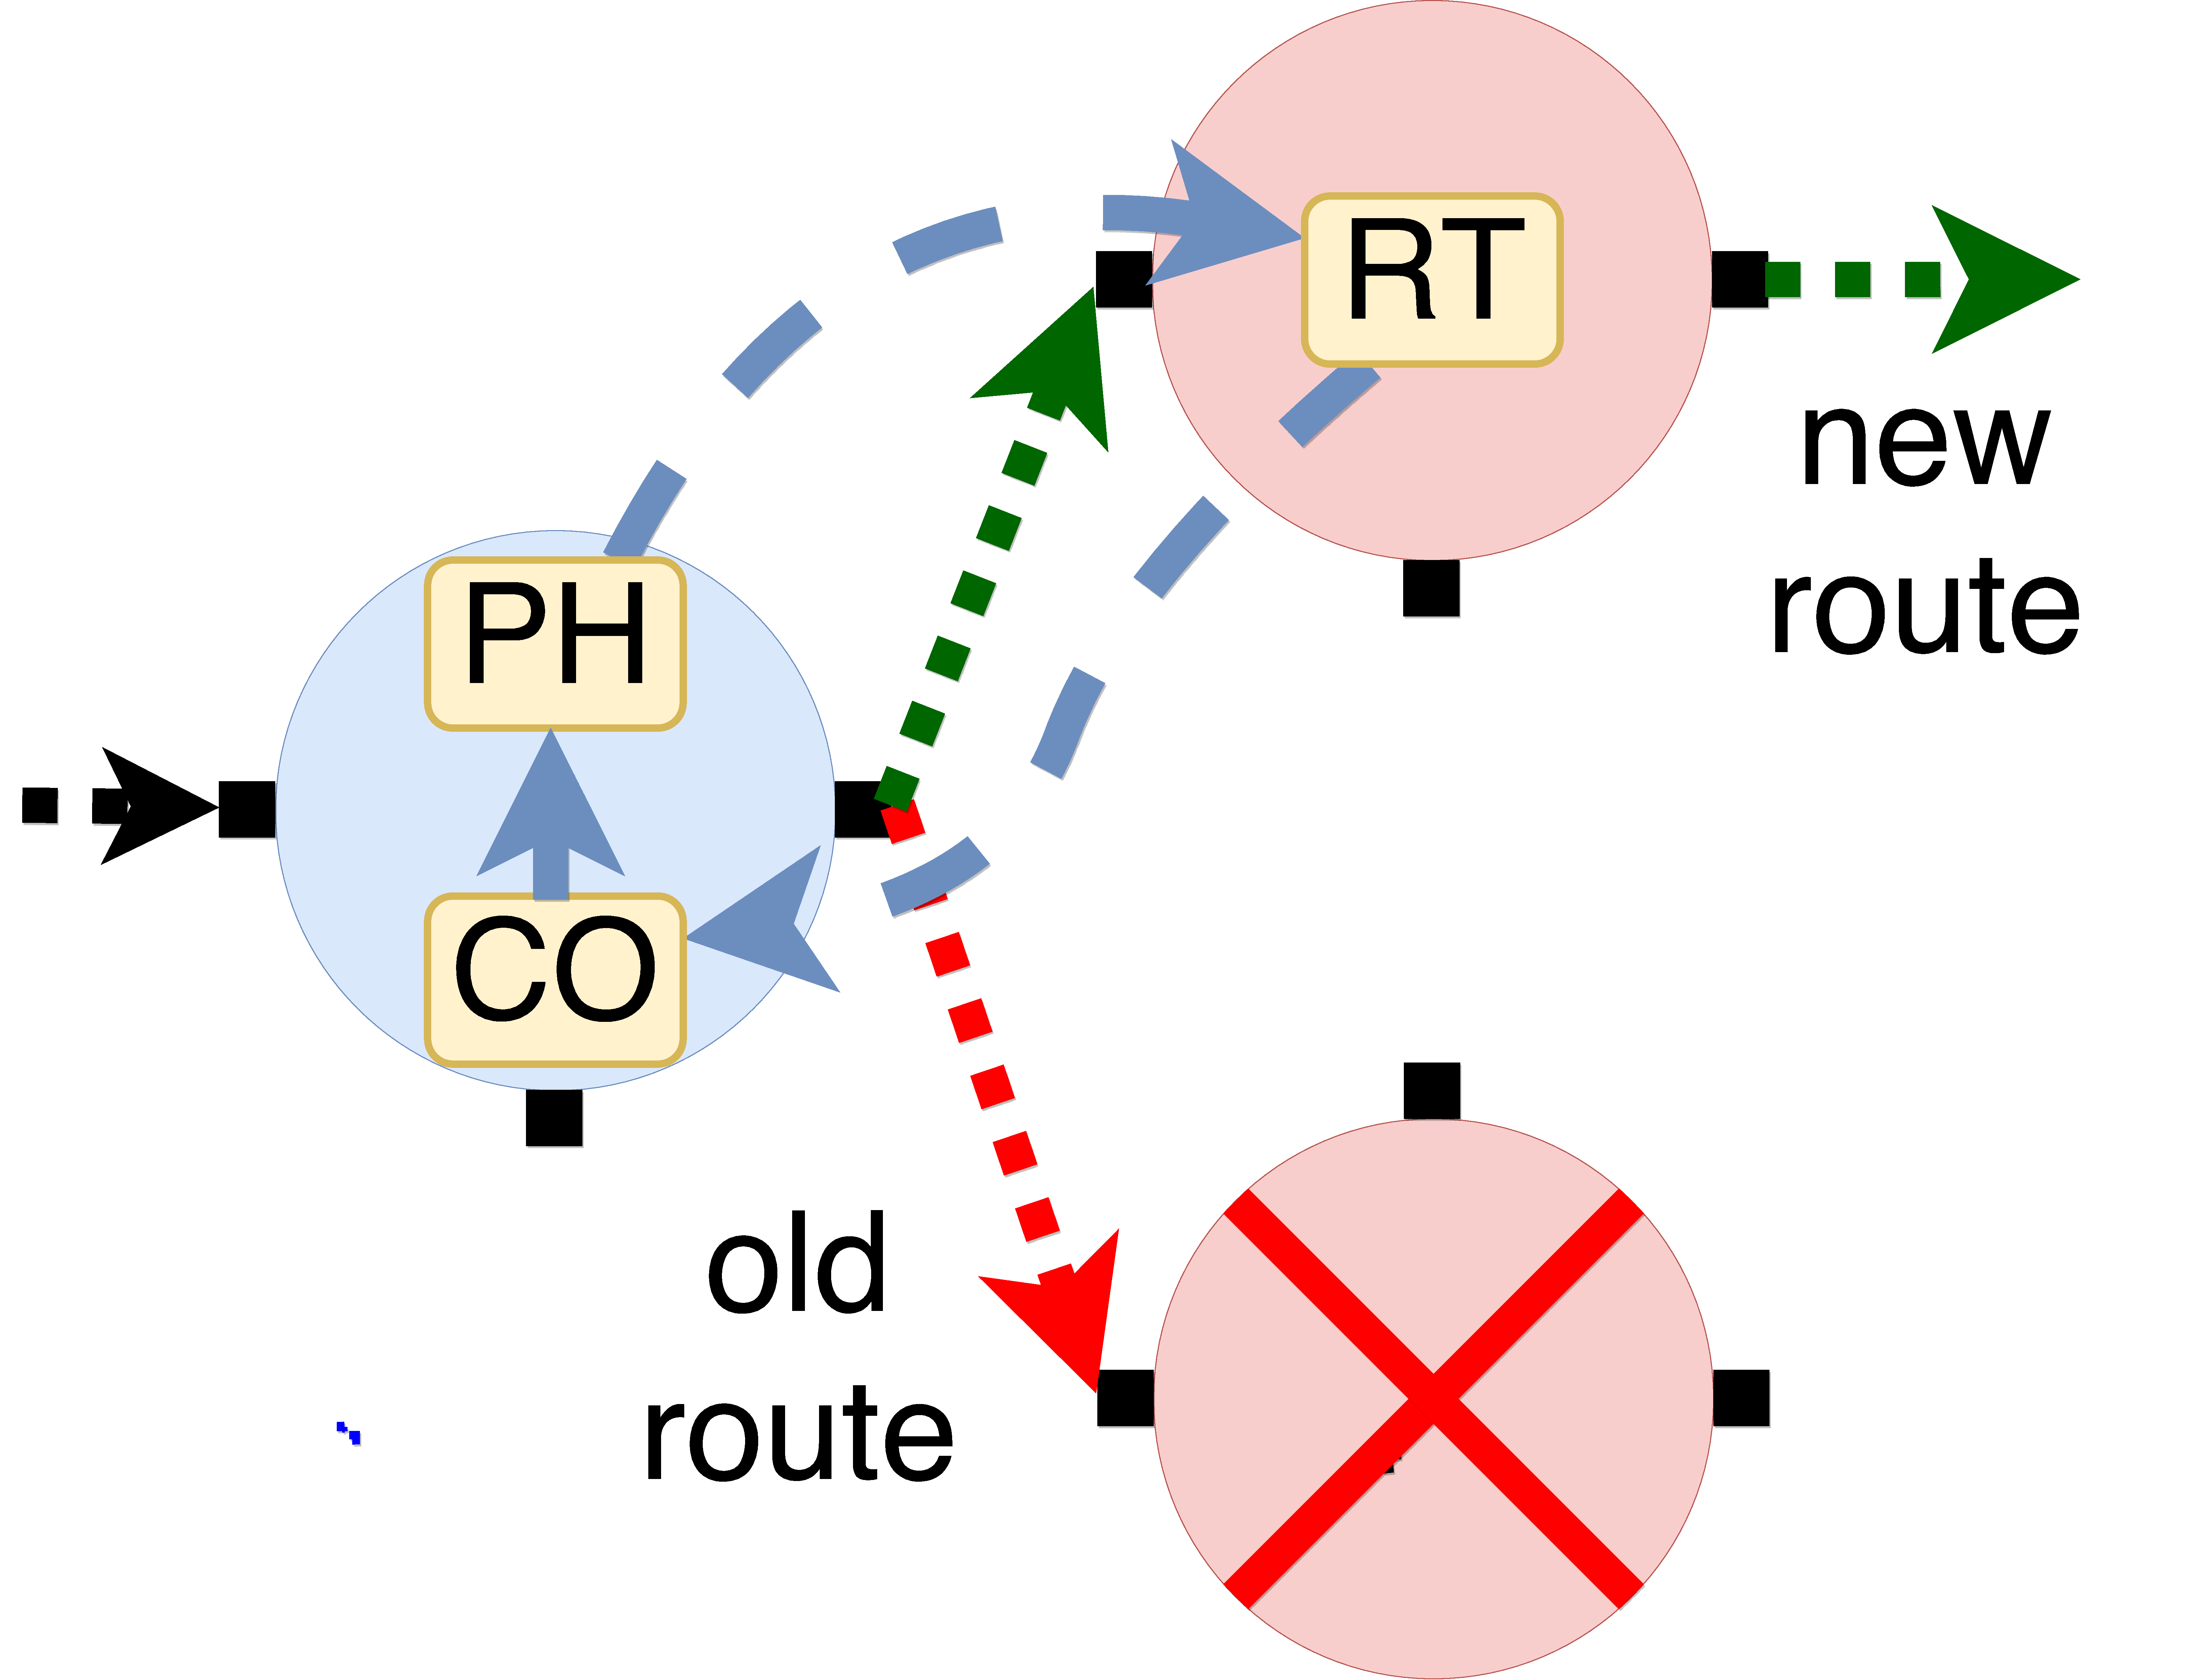
\includegraphics[width=0.66\columnwidth]{figure/nfactor-recover.pdf}
     \caption{Flow recover}\label{fig:recover}
    \end{subfigure}
 \caption{Flow replication and recover. (\textbf{RT}: Replication target actor. \textbf{RS}: Replication source actor. \textbf{CO}: Coordinator actor. \textbf{PH}: Flow actor on previous hop. \textbf{Dotted line}: Dataplane flow packets. \textbf{Dashed line}: Actor messages.)}
\label{fig:flow-rep}
\end{figure}

The biggest difference of the replication method used by NFActor and existing works such as \cite{sherry2015rollback} is that NFActor framework repliates individual flow, not NF. The reason that NFActor is able to replicate at such a fine granularity is because NFActor provides a fast execution context built using actor programming model and NFActor directly stores flow states inside each flow actor.

This replication strategy improves the scalability and resource utilization rate of the system. In NFActor, the flows could be directly replicated to another runtime within the same layer, without the need for a dedicated backup server. In the mean time, this fine grained replication strategy provides a strong replication consistency as indicated in \cite{sherry2015rollback} with a desirable performance.

The detailed flow replication process is shown in figure \ref{fig:flow-rep}. When a flow actor is created, it acquires its replica runtime by querying a round-rubin list. If the flow actor has a valid replica runtime, whenever it finishes processing the packet, it sends a remote message, containing the flow state and the packet, to the coordinator actor on the replication target runtime. The coorinator actor on the replication target runtime creates a replica flow actor using the same flow-5-tuple as the original flow actor to handle all the replication messages. The replica flow actor saves the flow state and sends the packet out from the output port of the replica runtime.

Similar with \cite{sherry2015rollback}, the receiver on the side of the output port of the replia runtime can only observe an output packet when the flow state has been replicated, which guarantes strong replication consistency.

When a runtime fails, the controller sends recovery RPC requests to all the replica runtime of the failed runtime. This RPC enables replica flow actor to send a route modification request to the previous hop flow actor. The previous hop flow actor then changes the output route to the replica runtime and gives a response back to the replica flow actor. When this request-response finishes, the original flow is recovered on the replica runtime.

\subsection{Alternative Design Option}

A runtime in NFActor framework is configured with a single service chain. Each flow is handled by a unique actor, which carries out all the processing on the configured service chain. Alternative design options do exist, however, they may not fully achieve our design goal to achieve low overhead and high scalability.

There are two alternatives to the one-flow-one-actor design. First of all, using a single flow actor to process multiple flows compromise the efficiency of flow migration protocol, especially when multiple flows come from different virtual switch actors. Under this situation, the flow actor must synchronize the responses sent from different virtual switch actors, therefore decreasing the performance of migration. Secondly, chaining several flow actors together to process the same flow imposes unnecessary overhead for flow processing. Therefore, the one-flow-one-actor design achieves a sweet point in minimizing the actor processing overhead and improving the efficiency of flow migration protocol design.

The alternative design to one-runtime-one-service-chain is to dynamically configure multiple service chains on a single runtime. Then due to the one-flow-one-actor design, we need to do an additional service chain selection, based on some pre-defined rules. This adds additional overhead to the flow actor processing and increases the complexity when managing the NFActor cluster, because the controller must populates the service chain rule dynamically to each runtime. With the one-runtime-on-service-chain design, if another service chain is needed, the system administrator could launch a new NFActor cluster and configure a different service chain to use.
